% !TeX root = memoria.tex
\documentclass{article}

\usepackage[spanish]{babel}

\usepackage[T1]{fontenc}
\usepackage[utf8]{inputenc}

\usepackage{graphicx}

\usepackage{amsmath}

\usepackage{float}

\usepackage{rotating} % Para la tabla horizontal
\usepackage{adjustbox} % Para ajustar el tamaño al ancho de página
\usepackage{array} % Para un mejor manejo de columnas

\usepackage{longtable}
\usepackage{amssymb}

\usepackage{geometry}
\geometry{a4paper, margin=1.5cm}

\usepackage{listings}
\usepackage{xcolor}

% Definición de colores
\definecolor{codegreen}{rgb}{0,0.6,0}
\definecolor{codegray}{rgb}{0.5,0.5,0.5}
\definecolor{codepurple}{rgb}{0.58,0,0.82}
\definecolor{backcolour}{rgb}{0.95,0.95,0.92}

% Estilo personalizado
\lstset{
    backgroundcolor=\color{backcolour},   
    commentstyle=\color{codegreen},
    keywordstyle=\color{blue},
    numberstyle=\tiny\color{codegray},
    stringstyle=\color{codepurple},
    basicstyle=\ttfamily\small,
    breakatwhitespace=false,         
    breaklines=true,                 
    captionpos=b,                    
    keepspaces=true,                 
    numbers=left,                    
    numbersep=5pt,                  
    showspaces=false,                
    showstringspaces=false,
    showtabs=false,                  
    tabsize=2,
    frame=single % Añade un marco alrededor del código
}

\title{MEMORIA PROCESADOR DE MYJS}
\date{\today}
\author{Acedo Blanco, Alvaro \\ Czepiel, Daniel \\ Grupo 96}

\begin{document}

\begin{figure}[t]
    \centering
    
\includegraphics[width=60pt]{./draco.png}
    \label{fig:draco}
\end{figure}

\maketitle
\tableofcontents

\newpage

\section{Diseño del analizador léxico}

\subsection{Tokens}a

Los tokens que usamos para el analizador léxico son:

\begin{center}
\begin{tabular}{c | c}
    \textbf{Codigo} & \textbf{Lexema} \\ \hline
    entero & valor \\
    real & valor \\
    cadena & lexema \\
    true & - \\
    false & - \\
    parentesis apertura & - \\
    parentersis cierre & - \\
    suma & - \\
    resta & - \\
    mayor & -\\
    mayor igual & - \\
    not & - \\
    and & - \\
    autodecremento & - \\
    asignacion & - \\
    identificador & posición tabla símbolos \\
    let & - \\
    int & - \\
    string & - \\
    boolean & - \\
    float & - \\
    void & - \\
    punto coma & - \\
    llave apertura & - \\
    llave cierre & - \\
    if & - \\
    else & - \\
    coma & - \\
    function & - \\
    read & - \\
    return & - \\
    write & - \\
    eof & - \\
\end{tabular}
\end{center}

Además se incluyo como token extra, el token error, que aunque como tal no sirve para representar ningún token de la gramática, a nivel de implementación nos ha sido útil tenerlo para poder representar casos como que todavía no se había leído un token.

\subsection{Gramática}

Donde el conjunto de terminales $T$ se define mediante la siguiente agrupación:

{\small
\[
T = \left\{ 
\begin{array}{ll}
\text{Alfanuméricos:} & \texttt{'a'-'z', 'A'-'Z', '0'-'9'} \text{ y el carácter subrayado (\_)} \\
\text{Blancos:} & \text{Espacio, Tabulador (TAB) y salto de línea (CR)} \\
\text{Operadores:} & \texttt{+, -, >, =, !, \&} \\
\text{Delimitadores:} & \texttt{(, ), \{, \}, ',', '.', ';', ", /} \\
\text{Especiales:} & \text{Carácter de escape (\textbackslash) y fin de fichero (EOF)}
\end{array} 
\right.
\]
}

El conjuto de los no terminales es: $N = \{S, A, B, C, D, E, F, G, H, I, J, K\}$

El axioma es: $S$ y las reglas de producción son:
\[ 
\begin{aligned}
P = \{ & S \to \text{EOF} \mid \; \text{del } S \mid \; d A \mid \; c D \mid \; \_ D \mid \; \text{\textquotedbl} E \mid \; ( \; \mid \; ) \mid \; + \mid \; - I \mid \; > G \mid \; \\
       & \mid \; ! \mid \; \& H \mid \; = \mid \; ; \mid \; \{ \; \mid \; \} \mid \; , \mid \; / J\\ \\
       & A \to d A \mid . B \mid \lambda \\
       & B \to d C \\
       & C \to d C \mid \lambda \\
       & D \to c D \mid _ D \mid d D \mid \lambda \\
       & E \to c_1 E \mid \text{\textbackslash} F \mid \text{\textquotedbl} \\
       & F \to n E \mid t E \\
       & G \to = \mid \lambda \\
       & H \to \& \\
       & I \to - \mid \lambda \\
       & J \to / K \\
       & K \to c_2 K \mid CR S \ EOF \\
\end{aligned}
\]

Siendo:
\[
    \begin{aligned}
        \text{del} &= \{\text{espacio, TAB, CR}\} \\
        c_1 &= T \text{\textbackslash} \{\text{\textbackslash, EOF, TAB, \textquotedbl}\} \\
        c_2 &= T \text{\textbackslash} \{\text{EOF, TAB}\}
    \end{aligned}
\]

\subsection{Diagrama del autómata y acciones semánticas}

Hicimos el siguiente autómata de la gramática regular:

\begin{figure}[H]
    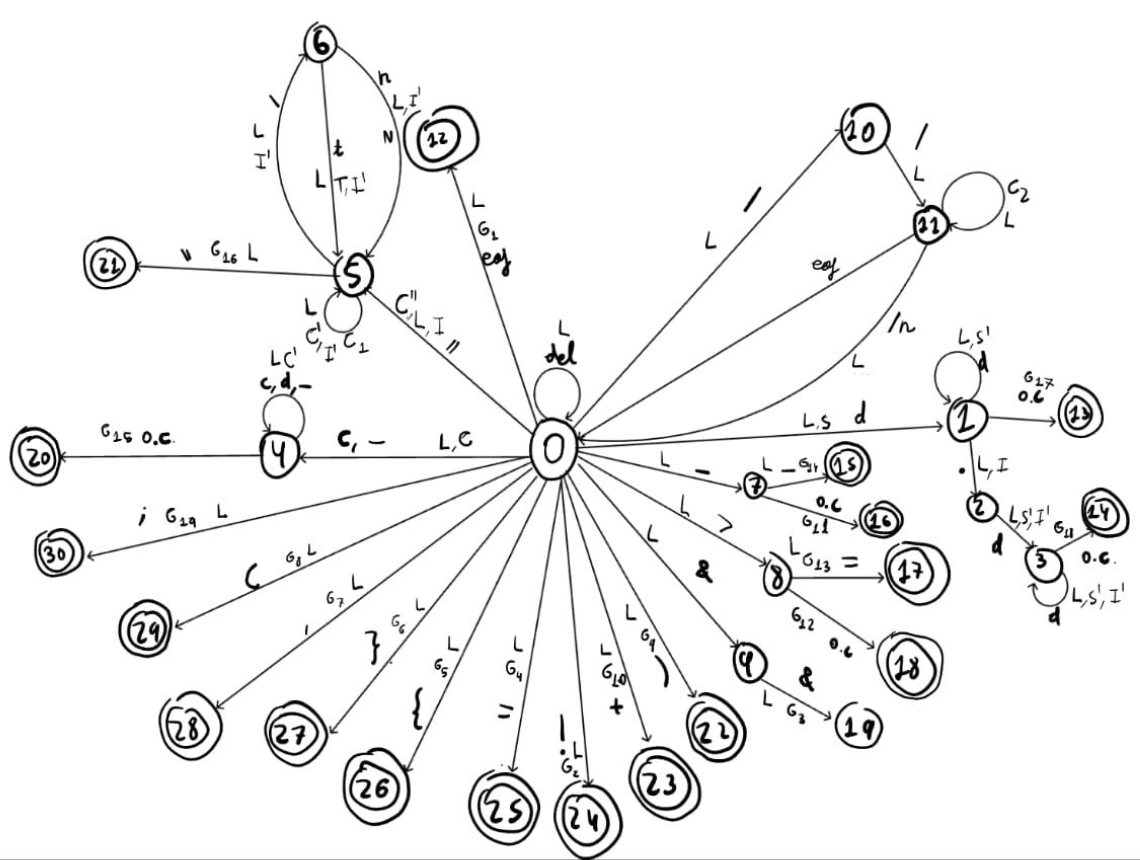
\includegraphics[width=325pt]{./AFD.png}
    \label{fig:afd}
\end{figure}
Las acciones semánticas son las siguientes:

\subsection{Descripción de las Acciones Semánticas}

A continuación se detallan todas las acciones semánticas ejecutadas por el autómata durante el proceso de análisis léxico:

\begin{description}
    \item[G1:] Generar Token $\langle$ eof, - $\rangle$
    \item[G2:] Generar Token $\langle$ not, - $\rangle$
    \item[G3:] Generar Token $\langle$ and, - $\rangle$
    \item[G4:] Generar Token $\langle$ asignación, - $\rangle$
    \item[G5:] Generar Token $\langle$ llaveApertura, - $\rangle$
    \item[G6:] Generar Token $\langle$ llaveCierre, - $\rangle$
    \item[G7:] Generar Token $\langle$ coma, - $\rangle$
    \item[G8:] Generar Token $\langle$ parentesisApertura, - $\rangle$
    \item[G9:] Generar Token $\langle$ parentesisCierre, - $\rangle$
    \item[G10:] Generar Token $\langle$ suma, - $\rangle$
    \item[G11:] Generar Token $\langle$ resta, - $\rangle$
    \item[G12:] Generar Token $\langle$ mayor, - $\rangle$
    \item[G13:] Generar Token $\langle$ mayorIgual, - $\rangle$
    \item[G14:] Generar Token $\langle$ autodecremento, - $\rangle$
    \item[G15:] \textbf{if} $p \neq$ null \textbf{then} \\
        \hspace*{1.5em} Generar Token $\langle$ PR\_p, - $\rangle$ \\
        \textbf{else} \\
        \hspace*{1.5em} $p = \text{BuscarTS}(\text{lexema})$ \\
        \hspace*{1.5em} \textbf{if} $p =$ null \textbf{then} \\
        \hspace*{3em} $p = \text{InsertarTS}(\text{lexema})$ \\
        \hspace*{1.5em} Generar Token $\langle$ identificador, $p$ $\rangle$
    \item[G16:] \textbf{if} cont $< 65$ \textbf{then} \\
        \hspace*{1.5em} Generar Token $\langle$ cadena, lexema $\rangle$ \\
        \textbf{else} \\
        \hspace*{1.5em} Error(28)
    \item[G17:] \textbf{if} $2^{15} > \text{num}$ \textbf{then} \\
        \hspace*{1.5em} Generar Token $\langle$ entero, num $\rangle$ \\
        \textbf{else} \\
        \hspace*{1.5em} Error(21)
    \item[G18:] num = num $\times 10^{-\text{cont}}$ \\
        \textbf{if} num $<$ NUM\_MAX \textbf{then} \\
        \hspace*{1.5em} Generar Token $\langle$ real, num $\rangle$ \\
        \textbf{else} \\
        \hspace*{1.5em} Error(24)
    \item[G19:] Generar Token $\langle$ puntoComa, - $\rangle$
    \item[L:] $car = \text{leer}()$
    \item[C:] lexema = caracter
    \item[C':] lexema = lexema + caracter
    \item[C'':] lexema = ""; cont = 0
    \item[N:] lexema = lexema + '\textbackslash n'
\end{description}

\subsection{Errores}
Para los errores hemos tenido en cuenta:

\begin{itemize}
    \item Caracter desconocido
    \item El uso incorrecto de comentarios. Del tipo //
    \item El uso incorrecto del operador and
    \item La terminación de las cadenas
    \item Secuencias de escape correctas
    \item Números reales bien formados
    \item Esceso de bytes para un tipo de dato
\end{itemize}

Al encontrarse el analizador léxico con un error este lo que hace es llamar a
una función que se encarga de meter en pila el error con su código y mensaje
de error.
\newpage

\section{Diseño del analizador sintáctico}

\subsection{Gramática}

Para la gramática hemos utilizado una gramática descendente tabular. Esta tiene la siguiente forma:

El conjunto de de símbolos no terminales es: 

NoTerminales $= \{A, B, C, D, E, E1, F, G, H, I, K, L, O, P, Q, R, R1, S, T,$

$U, U1, V, W, X, Z \}$

El axioma es:

Axioma $= P$

\[ \text{Producciones } P = \{ \]
\begin{minipage}[t]{0.45\textwidth}
\small
\[ \begin{aligned}
    &E \to R E' && \text{(R1)} \\
    &E' \to \&\& R E' && \text{(R2)} \\
    &E' \to \lambda && \text{(R3)} \\
    &R \to U R' \\
    &R' \to > U R' && \text{(R5)} \\
    &R' \to >= U R' \\
    &R' \to \lambda \\
    &U \to V U' \\
    &U' \to + V U' \\
    &U' \to - V U' && \text{(R10)} \\
    &U' \to \lambda \\
    &V \to + W  \\
    &V \to - W \\
    &V \to ! W \\
    &V \to -- W  && \text{(R15)} \\
    &V \to W \\
    &W \to \text{id } O \\
    &W \to ( E ) \\
    &W \to \text{entero} \\
    &W \to \text{real}  && \text{(R20)} \\
    &W \to \text{cadena} \\
    &W \to \text{true} \\
    &W \to \text{false} \\
    &O \to ( L ) \\
    &O \to \lambda  && \text{(R25)}
\end{aligned} \]
\end{minipage}
\hfill
\begin{minipage}[t]{0.45\textwidth}
\small
\[ \begin{aligned}
    &S \to \text{id } G ; \\
    &S \to \text{write } E ; \\
    &S \to \text{read id} ; \\
    &S \to \text{return } X ; \\
    &G \to = E && \text{(R30)}  \\
    &G \to ( L ) \\
    &L \to E Q  \\
    &L \to \lambda \\
    &Q \to , E Q \\
    &Q \to \lambda && \text{(R35)} \\
    &X \to E \\
    &X \to \lambda \\
    &B \to \text{if } ( E ) Z \\
    &Z \to S \\
    &Z \to \{ C \} I && \text{(R40)} \\
    &I \to \text{else } D \\
    &I \to \lambda \\
    &D \to \text{if } ( E ) \{ C \} I \\
    &D \to \{ C \} \\
    &B \to \text{let } T \text{ id} ; && \text{(R45)} \\
    &B \to S \\
    &T \to \text{int} \\
    &T \to \text{float} \\
    &T \to \text{boolean} \\
    &T \to \text{string} && \text{(R50)}
\end{aligned} \]
\end{minipage}

\[ \begin{aligned}
    &F \to \text{function } H \text{ id } ( A ) \{ C \} && \text{(R51)} \\
    &H \to T \\
    &H \to \text{void} \\
    &A \to T \text{ id } K \\
    &A \to \text{void} && \text{(R55)} \\
    &K \to , T \text{ id } K \\
    &K \to \lambda \\
    &C \to B C \\
    &C \to \lambda \\
    &P \to B P && \text{(R60)} \\
    &P \to F P \\
    &P \to \lambda && \text{(R62)}
\end{aligned} \]

\subsection{Tabla}
Se adjunta en la siguiente página la tabla del analizador sintáctico por mótivos de su tamaño, está en su propia página y dada la vuelta para poder caber mejor.

Se tuvo que calcular el follow y next de las reglas para poder hacerla, y la tabla demuestra que la gramática es LL(1), ya que, de no serlo deberían de coincidir en la misma 
casilla dos o más reglas.

\begin{sidewaystable}[p]
    \centering
    \caption{Tabla de Análisis Sintáctico LL(1) - Transcripción Literal}
    \label{tab:sintactica_literal}
    \begin{adjustbox}{width=\textwidth}
    \tiny
    \begin{tabular}{|c|c|c|c|c|c|c|c|c|c|c|c|c|c|c|c|c|c|c|c|c|c|c|c|c|c|c|c|c|c|c|c|c|c|}
    \hline
    & \textbf{entero} & \textbf{real} & \textbf{ccadena} & \textbf{true} & \textbf{false} & \textbf{pA} & \textbf{pC} & \textbf{suma} & \textbf{resta} & \textbf{>} & \textbf{>=} & \textbf{!} & \textbf{\&\&} & \textbf{--} & \textbf{=} & \textbf{id} & \textbf{let} & \textbf{int} & \textbf{string} & \textbf{boolean} & \textbf{float} & \textbf{void} & \textbf{;} & \textbf{llaveA} & \textbf{llaveC} & \textbf{if} & \textbf{else} & \textbf{coma} & \textbf{function} & \textbf{read} & \textbf{return} & \textbf{write} & \textbf{\$} \\ \hline
    
    \textbf{A} & & & & & & & & & & & & & & & & & & $A \to T id K$ & $A \to T id K$ & $A \to T id K$ & $A \to T id K$ & $A \to void$ & & & & & & & & & & & \\ \hline
    \textbf{B} & & & & & & & & & & & & & & & & $B \to S$ & $B \to let T id;$ & & & & & & & & $B \to if ( E ) Z$ & & & & $B \to S$ & $B \to S$ & $B \to S$ & \\ \hline
    \textbf{C} & & & & & & & & & & & & & & & & $C \to B C$ & $C \to B C$ & & & & & & & $C \to \lambda$ & $C \to B C$ & & & & $C \to B C$ & $C \to B C$ & $C \to B C$ & \\ \hline
    \textbf{D} & & & & & & & & & & & & & & & & & & & & & & & & $D \to \{ C \}$ & & $D \to if ( E ) \{ C \}$ & & & & & & & \\ \hline
    \textbf{E} & $E \to R E'$ & $E \to R E'$ & $E \to R E'$ & $E \to R E'$ & $E \to R E'$ & $E \to R E'$ & & & & & & & & & & $E \to R E'$ & & & & & & & & & & & & & & & & & \\ \hline
    \textbf{E'} & & & & & & & $E' \to \lambda$ & & & & & & $E' \to \&\& R E'$ & & & & & & & & & & $E' \to \lambda$ & & $E' \to \lambda$ & & $E' \to \lambda$ & $E' \to \lambda$ & & & & & $E' \to \lambda$ \\ \hline
    \textbf{F} & & & & & & & & & & & & & & & & & & & & & & & & & & & & & $F \to function H id ( A ) \{ C \}$ & & & & \\ \hline
    \textbf{G} & & & & & & & $G \to ( L )$ & & & & & & & & $G \to = E$ & & & & & & & & & & & & & & & & & & \\ \hline
    \textbf{H} & & & & & & & & & & & & & & & & & & $H \to T$ & $H \to T$ & $H \to T$ & $H \to T$ & $H \to void$ & & & & & & & & & & & \\ \hline
    \textbf{I} & & & & & & & & & & & & & & & & $I \to \lambda$ & $I \to \lambda$ & & & & & & & & $I \to \lambda$ & $I \to \lambda$ & $I \to else D$ & & $I \to \lambda$ & $I \to \lambda$ & $I \to \lambda$ & $I \to \lambda$ & $I \to \lambda$ \\ \hline
    \textbf{K} & & & & & & & $K \to \lambda$ & & & & & & & & & & & & & & & & & & & & & $K \to , T id K$ & & & & & \\ \hline
    \textbf{L} & $L \to E Q$ & $L \to E Q$ & $L \to E Q$ & $L \to E Q$ & $L \to E Q$ & $L \to E Q$ & $L \to \lambda$ & & & & & & & & & $L \to E Q$ & & & & & & & & & & & & & & & & & \\ \hline
    \textbf{P} & & & & & & & & & & & & & & & & $P \to B P$ & $P \to B P$ & & & & & & & & & $P \to B P$ & & & $P \to F P$ & $P \to B P$ & $P \to B P$ & $P \to B P$ & $P \to \lambda$ \\ \hline
    \textbf{Q} & & & & & & & $Q \to \lambda$ & & & & & & & & & & & & & & & & & & & & & $Q \to , E Q$ & & & & & \\ \hline
    \textbf{R} & $R \to U R'$ & $R \to U R'$ & $R \to U R'$ & $R \to U R'$ & $R \to U R'$ & $R \to U R'$ & & & & & & & & & & $R \to U R'$ & & & & & & & & & & & & & & & & & \\ \hline
    \textbf{R'} & & & & & & & $R' \to \lambda$ & & & $R' \to > U R'$ & $R' \to >= U R'$ & & $R' \to \lambda$ & & & & & & & & & & $R' \to \lambda$ & & $R' \to \lambda$ & & $R' \to \lambda$ & $R' \to \lambda$ & & & & & $R' \to \lambda$ \\ \hline
    \textbf{S} & & & & & & & & & & & & & & & & $S \to id G ;$ & & & & & & & & & & & & & & $S \to read id ;$ & $S \to return X ;$ & $S \to write E ;$ & \\ \hline
    \textbf{T} & & & & & & & & & & & & & & & & & & $T \to int$ & $T \to string$ & $T \to boolean$ & $T \to float$ & & & & & & & & & & & & \\ \hline
    \textbf{U} & $U \to V U'$ & $U \to V U'$ & $U \to V U'$ & $U \to V U'$ & $U \to V U'$ & $U \to V U'$ & & & & & & & & & & $U \to V U'$ & & & & & & & & & & & & & & & & & \\ \hline
    \textbf{U'} & & & & & & & $U' \to \lambda$ & $U' \to + V R'$ & $U' \to - V R'$ & $U' \to \lambda$ & $U' \to \lambda$ & & $U' \to \lambda$ & & & & & & & & & & $U' \to \lambda$ & & $U' \to \lambda$ & & $U' \to \lambda$ & $U' \to \lambda$ & & & & & $U' \to \lambda$ \\ \hline
    \textbf{V} & $V \to W$ & $V \to W$ & $V \to W$ & $V \to W$ & $V \to W$ & $V \to W$ & & $V \to + W$ & $V \to - W$ & & & $V \to ! W$ & & $V \to -- W$ & & $V \to W$ & & & & & & & & & & & & & & & & & \\ \hline
    \textbf{W} & $W \to entero$ & $W \to real$ & $W \to cadena$ & $W \to true$ & $W \to false$ & $W \to ( E )$ & & & & & & & & & & $W \to id O$ & & & & & & & & & & & & & & & & & \\ \hline
    \textbf{X} & $X \to E$ & $X \to E$ & $X \to E$ & $X \to E$ & $X \to E$ & $X \to E$ & & & & & & & & & & $X \to E$ & & & & & & & $X \to \lambda$ & & & & & & & & & & \\ \hline
    \textbf{Z} & & & & & & & & & & & & & & & & $Z \to S$ & & & & & & & & $Z \to \{ C \} Z$ & & & & & & $Z \to S$ & $Z \to S$ & $Z \to S$ & \\ \hline
    \end{tabular}
    \end{adjustbox}
\end{sidewaystable}

\subsection{Errores}
Para los errores hemos tenido en cuenta:

\begin{itemize}
    \item Errores al leer terminales no esperados
    \item Empezar mal una sentencia
    \item No poner los atributos de una función
    \item Declarar de forma incorrecta una función
    \item No terminar la asignación de una variable
    \item Expresiones con operandos incorrectas
    \item El cierre correcto del archivo con un final de bloque o de sentencia
\end{itemize}
\newpage

\section{Diseño del analizador semántico}
Hemos utilizado el siguiente EdT:

\renewcommand{\arraystretch}{1.6} % Mejora la separación entre reglas

% Usamos p{ancho} directamente para evitar errores de "Illegal pream-token"
% El comando >{\raggedright\arraybackslash} asegura que el texto no se justifique feo
\begin{longtable}{|c|>{\raggedright\arraybackslash}p{5.5cm}|>{\raggedright\arraybackslash}p{10cm}|}
\hline
\textbf{\#} & \textbf{Producción} & \textbf{Acciones Semánticas} \\ \hline
\endhead

\hline
\multicolumn{3}{|r|}{\textit{Continúa en la siguiente página...}} \\
\hline
\endfoot

\hline
\endlastfoot

% Regla 1
1 & $E \to R \; E_1$ & 
$E.tipo = \texttt{if}(E_1.tipo == \texttt{void} \lor R.tipo == E_1.tipo)$ \newline
\hspace*{0.5cm} $\texttt{then } R.tipo$ \newline
\hspace*{0.5cm} $\texttt{else tipo\_error}$ \newline
\texttt{\{AUX -= 2\}} \\ \hline

% Regla 2
2 & $E_1 \to \&\& \; R \; E_{1\_1}$ & 
$E_1.tipo = \texttt{if}(R.tipo == \texttt{logico} \land E_{1\_1}.tipo \in \{\texttt{logico, void}\})$ \newline
\hspace*{0.5cm} $\texttt{then } R.tipo$ \newline
\hspace*{0.5cm} $\texttt{else tipo\_error}$ \newline
\texttt{\{AUX -= 3\}} \\ \hline

% Regla 3
3 & $E_1 \to \lambda$ & 
$E_1.tipo = \texttt{void}$ \newline
\texttt{\{AUX -= 0\}} \\ \hline

% Regla 4
4 & $R \to U \; R_1$ & 
$R.tipo = \texttt{if}(R_1.tipo == \texttt{void}) \texttt{ then } U.tipo$ \newline
\hspace*{0.5cm} $\texttt{else if}(U.tipo == R_1.tipo) \texttt{ then logico}$ \newline
\hspace*{0.5cm} $\texttt{else tipo\_error}$ \newline
\texttt{\{AUX -= 2\}} \\ \hline

% Regla 5
5 & $R_{1\_1} \to > \; U \; R_{1\_2}$ & 
$R_{1\_1}.tipo = \texttt{if}(U.tipo \in \{\texttt{real, entero}\} \land R_{1\_2} == \texttt{void})$ \newline
\hspace*{0.5cm} $\texttt{then } U.tipo$ \newline
\hspace*{0.5cm} $\texttt{else tipo\_error}$ \newline
\texttt{\{AUX -= 3\}} \\ \hline

% Regla 6
6 & $R_{1\_1} \to \ge \; U \; R_{1\_2}$ & 
$R_{1\_1}.tipo = \texttt{if}(U.tipo \in \{\texttt{real, entero}\} \land R_{1\_2} == \texttt{void})$ \newline
\hspace*{0.5cm} $\texttt{then } U.tipo$ \newline
\hspace*{0.5cm} $\texttt{else tipo\_error}$ \newline
\texttt{\{AUX -= 3\}} \\ \hline

% Regla 7
7 & $R_1 \to \lambda$ & 
$R_1.tipo = \texttt{void}$ \newline
\texttt{\{AUX -= 0\}} \\ \hline

% Regla 8
8 & $U \to V \; U_1$ & 
$U.tipo = \texttt{if}(U_1.tipo == \texttt{void} \lor V.tipo == U_1.tipo)$ \newline
\hspace*{0.5cm} $\texttt{then } V.tipo$ \newline
\hspace*{0.5cm} $\texttt{else tipo\_error}$ \newline
\texttt{\{AUX -= 2\}} \\ \hline

% Regla 9
9 & $U_1 \to + \; V \; U_{1\_1}$ & 
$U_1.tipo = \texttt{if}((V.tipo \in \{\texttt{entero, real}\} \land U_{1\_1}.tipo == \texttt{void}) \lor V.tipo == U_{1\_1}.tipo)$ \newline
\hspace*{0.5cm} $\texttt{then } V.tipo$ \newline
\hspace*{0.5cm} $\texttt{else tipo\_error}$ \newline
\texttt{\{AUX -= 3\}} \\ \hline

% Regla 10
10 & $U_1 \to - \; V \; U_{1\_1}$ & 
$U_1.tipo = \texttt{if}((V.tipo \in \{\texttt{entero, real}\} \land U_{1\_1}.tipo == \texttt{void}) \lor V.tipo == U_{1\_1}.tipo)$ \newline
\hspace*{0.5cm} $\texttt{then } V.tipo$ \newline
\hspace*{0.5cm} $\texttt{else tipo\_error}$ \newline
\texttt{\{AUX -= 3\}} \\ \hline

% Regla 11
11 & $U_1 \to \lambda$ & 
$U_1.tipo = \texttt{void}$ \newline
\texttt{\{AUX -= 0\}} \\ \hline

% Regla 12
12 & $V \to + \; W$ & 
$V.tipo = \texttt{if}(W.tipo \in \{\texttt{entero, real}\}) \texttt{ then } W.tipo$ \newline
\hspace*{0.5cm} $\texttt{else tipo\_error}$ \newline
\texttt{\{AUX -= 2\}} \\ \hline

% Regla 13
13 & $V \to - \; W$ & 
$V.tipo = \texttt{if}(W.tipo \in \{\texttt{entero, real}\}) \texttt{ then } W.tipo$ \newline
\hspace*{0.5cm} $\texttt{else tipo\_error}$ \newline
\texttt{\{AUX -= 2\}} \\ \hline

% Regla 14
14 & $V \to ! \; W$ & 
$V.tipo = \texttt{if}(W.tipo == \texttt{lógico}) \texttt{ then tipo\_logico}$ \newline
\hspace*{0.5cm} $\texttt{else tipo\_error}$ \newline
\texttt{\{AUX -= 2\}} \\ \hline

% Regla 15
15 & $V \to -- \; \mathbf{id}$ & 
$V.tipo = \texttt{if}(\text{buscarTipo}(\mathbf{id}.pos) \in \{\texttt{real, entero}\})$ \newline
\hspace*{0.5cm} $\texttt{then } \text{buscarTipo}(\mathbf{id}.pos)$ \newline
\hspace*{0.5cm} $\texttt{else tipo\_error}$ \newline
\texttt{\{AUX -= 2\}} \\ \hline

% Regla 16
16 & $V \to W$ & 
$V.tipo = W.tipo$ \newline
\texttt{\{AUX -= 1\}} \\ \hline

% Regla 17
17 & $W \to \mathbf{id} \; O$ & 
$W.tipo = \texttt{if}(O.tipo == \texttt{void}) \texttt{ then } \text{buscarTipo}(\mathbf{id}.pos)$ \newline
\hspace*{0.5cm} $\texttt{else if}(\text{buscarParam}(\mathbf{id}.pos) == O.parametros)$ \newline
\hspace*{1cm} $\texttt{then } \text{buscarTipoRet}(\mathbf{id}.pos)$ \newline
\hspace*{1cm} $\texttt{else tipo\_error}$ \newline
\texttt{\{AUX -= 2\}} \\ \hline

% Regla 18
18 & $W \to ( \; E \; )$ & 
$W.tipo = E.tipo$ \newline
\texttt{\{AUX -= 3\}} \\ \hline

% Regla 19, 20, 21, 22, 23
19 & $W \to \texttt{entero}$ & $W.tipo = \texttt{entero}$ \hspace{1cm} \texttt{\{AUX -= 1\}} \\ \hline
20 & $W \to \texttt{real}$ & $W.tipo = \texttt{real}$ \hspace{1.2cm} \texttt{\{AUX -= 1\}} \\ \hline
21 & $W \to \texttt{cadena}$ & $W.tipo = \texttt{cadena}$ \hspace{0.9cm} \texttt{\{AUX -= 1\}} \\ \hline
22 & $W \to \texttt{true}$ & $W.tipo = \texttt{lógico}$ \hspace{1cm} \texttt{\{AUX -= 1\}} \\ \hline
23 & $W \to \texttt{false}$ & $W.tipo = \texttt{lógico}$ \hspace{1cm} \texttt{\{AUX -= 1\}} \\ \hline

% Regla 24
24 & $O \to ( \; L \; )$ & 
$O.tipo = \texttt{tipo\_funcion}$ \newline
$O.parametros = L.parametros$ \newline
$O.numParam = L.numeroParametros$ \newline
\texttt{\{AUX -= 3\}} \\ \hline

% Regla 25
25 & $O \to \lambda$ & 
$O.tipo = \texttt{void}$ \newline
\texttt{\{AUX -= 0\}} \\ \hline

% Regla 26
26 & $S \to \mathbf{id} \; G \; ;$ & 
$S.tipo = \texttt{if}(\text{buscarTipo}(\mathbf{id}.pos) == G.tipo == \texttt{tipo\_funcion})$ \newline
\hspace*{0.5cm} $\texttt{then if}(\text{buscarParam}(\mathbf{id}.pos) \neq G.parametros) \texttt{ tipo\_error}$ \newline
\hspace*{0.5cm} $\texttt{else if}(\text{buscarTipo}(\mathbf{id}.pos) \neq G.tipo) \texttt{ then tipo\_error}$ \newline
\texttt{\{AUX -= 3\}} \\ \hline

% Regla 27
27 & $S \to \texttt{write} \; E \; ;$ & 
$S.tipo = \texttt{if}(E.tipo \notin \{\texttt{entero, real, cadena}\}) \texttt{ then tipo\_error}$ \newline
$S.tipoRet = \texttt{void}$ \newline
\texttt{\{AUX -= 3\}} \\ \hline

% Regla 28
28 & $S \to \texttt{read} \; \mathbf{id} \; ;$ & 
$S.tipo = \texttt{if}(\text{buscarTipoTS}(\mathbf{id}.pos) \notin \{\texttt{entero, real, cadena}\})$ \newline
\hspace*{0.5cm} $\texttt{then tipo\_error}$ \newline
$S.tipoRet = \texttt{void}$ \newline
\texttt{\{AUX -= 3\}} \\ \hline

% Regla 29
29 & $S \to \texttt{return} \; X \; ;$ & 
$S.tipo = \texttt{if}(X.tipo \neq S.tipoRet) \texttt{ then tipo\_error}$ \newline
\texttt{\{AUX -= 3\}} \\ \hline

% Regla 30
30 & $G \to = \; E$ & 
$G.tipo = E.tipo$ \newline
\texttt{\{AUX -= 2\}} \\ \hline

% Regla 31
31 & $G \to ( \; L \; )$ & 
$G.tipo = \texttt{tipo\_funcion}$ \newline
$G.parametros = L.parametros, G.numParam = L.numParametros$ \newline
\texttt{\{AUX -= 3\}} \\ \hline

% Regla 32, 33, 34, 35
32 & $L \to E \; Q$ & $L.param = E.tipo \times Q.param, L.numP = 1 + Q.numP$ \newline \texttt{\{AUX -= 2\}} \\ \hline
33 & $L \to \lambda$ & $L.param = \texttt{void}, L.numP = 0$ \hspace{1cm} \texttt{\{AUX -= 0\}} \\ \hline
34 & $Q_1 \to , \; E \; Q_2$ & $Q_1.param = E.tipo \times Q_2.param, Q_1.numP = 1 + Q_2.numP$ \newline \texttt{\{AUX -= 3\}} \\ \hline
35 & $Q \to \lambda$ & $Q.param = \texttt{void}, Q.numP = 0$ \hspace{1cm} \texttt{\{AUX -= 0\}} \\ \hline

% Regla 38, 39 (IF)
38, 39 & $B \to \texttt{if} \; ( \; E \; ) \; Z$ & 
$B.tipo = \texttt{if}(E.tipo == \texttt{logico}) \texttt{ then tipo\_error}$ \newline
$B.tipoRet = Z.tipoRet$ \newline
\texttt{\{AUX -= 5\}} \\ \hline

% Regla 51, 52 (LET)
51, 52 & $B \to \texttt{let} \; T \; \mathbf{id} \; ;$ & 
$\texttt{zonaDecl = true}$ \newline
$\text{añadirTipo}(\mathbf{id}.pos, T.tipo)$ \newline
$\text{añadirDespl}(\mathbf{id}.pos, despl)$ \newline
$\text{desplazamiento} += T.\text{tamaño}$ \newline
$\texttt{zonaDecl = false}$ \newline
\texttt{\{AUX -= 4\}} \\ \hline

% Regla 58, 59, 60 (Function)
58-60 & $F \to \texttt{function} \; H \; \mathbf{id} \; ( \; A \; ) \; \{ \; C \; \}$ & 
$\texttt{zonaDecl = true}, \text{añadeTipo}(\mathbf{id}.pos, \texttt{tipo\_func})$ \newline
$\text{añadeTipoRet}(\mathbf{id}.pos, H.tipo), C.tipoRet = H.tipo$ \newline
$\text{añadeEtiq}(\mathbf{id}.pos, \text{nuevaEtiq}())$ \newline
$TSF = \text{crearTabla}(), \text{despl} = 0, \texttt{zonaDecl = false}$ \newline
$\text{añadeParam}(\mathbf{id}.pos, A.param), \text{liberarTabla}(TSF)$ \newline
\texttt{\{AUX -= 9\}} \\ \hline

% Regla 68, 69 (Programa Principal)
68, 69 & $PP \to P$ & 
$TS = \text{crearTabla}(), \text{desplazamiento} = 0$ \newline
$\text{liberarTabla}(TS)$ \newline
\texttt{\{AUX -= 1\}} \\ \hline

\end{longtable}

\newpage
\subsection{Errores}
Para los errores hemos tenido en cuenta:

\begin{itemize}
    \item El uso de tipos correctos en expresiones como and o >
    \item La no conversión de tipo en operaciones
    \item La utilización de llamadas a funciones con el número y el tipo correctos de los parámetros\
    \item La asignación de variables con datos del mismo tipo
    \item Utilización de write y read con variables de tipo entero, real o cadena
    \item El tipo devuelto en funciones
    \item Que las sentencias de comprobación del if sean de tipo lógico
\end{itemize}
\newpage

\section{Diseño de la tabla de símbolos}
En la tabla de símbolos hemos utilizado la busqueda lineal para recorrer las tablas.

Hemos diferenciado las posiciones de la tabla de símbolos global de las de la función denotando las posiciones de la tabla de función negativas y haciendo que la primera
posición de cada tabla sea 1 y -1 respectivamente.
\newpage

\section{Diseño del gestor de errores}
Para el gestor de errores hemos decidido hacer recuperación de errores, así el gestor recopila los errores del archivo entero y luego los vuelca una vez terminado de analizar el fichero entero.

Para el contéo del número de línea, creamos una función la cual el analizador léxico llama cada vez que lee el delimitador salto de línea.
\newpage

\section{Anexo: ficheros de prueba}

El lenguaje que elegimos para hacer la práctia es C, el cual te obliga a hacer gestión de la memoria dinámica. Hemos tenido en la implementación final varios errores de memoria.

\subsection{Ficheros correctos}

\subsubsection{Fichero 1}

\begin{lstlisting}[language=Java, title={fichero1.txt}]
    let int a ;
    let  float   b  ;
    let boolean bbb ;
    a = a - c;
    write a ;
    write b;
    write ccc;
\end{lstlisting}

Da un error de memoria el procesador al intentar ejecutar el fichero

TablaTokens:

TablaSimbolos:

Parse:

\subsubsection{Fichero 2}
\begin{lstlisting}[language=Java, title={fichero2.txt}]
    let int x; function float hola (int hola){}
hola(x);
function void hola2(float f, boolean b){
    let int i;
    hola(--i);
    hola(-i);
    return ;
}

let boolean y;
hola2(hola(x),y); 



\end{lstlisting}

Da un error de memoria el procesador al intentar ejecutar el fichero

TablaTokens:

TablaSimbolos:

Parse:


\subsubsection{Fichero 3}
\begin{lstlisting}[language=Java, title={fichero3.txt}]
function string hello(void){
    let string hola = "hola";
    write hola;
    if(true){
        return hola;
    }
    else{
        return hello();
    }
}
\end{lstlisting}

Da un error de memoria el procesador al intentar ejecutar el fichero

TablaTokens:

TablaSimbolos:

Parse:


\subsubsection{Fichero 4}
\begin{lstlisting}[language=Java, title={fichero4.txt}]
  let boolean a;
let boolean b;
a = 3 &&( 4 > (2 + 1) )&& !true;
b=a;
let float rrr;
let float ccc;if (rrr >= ccc) b = false;
  
\end{lstlisting}


TablaTokens:

TablaSimbolos:

Arbol de derivación: \vspace{2ex}
PP

\hspace{2ex} P

\hspace{4ex} B

\hspace{8ex} let

\hspace{8ex} T

\hspace{16ex} boolean

\hspace{8ex} id

\hspace{8ex} ;

\hspace{2ex} P

\hspace{4ex} B

\hspace{8ex} let

\hspace{8ex} T

\hspace{16ex} boolean

\hspace{8ex} id

\hspace{8ex} ;

\hspace{4ex} P

\hspace{8ex} B

\hspace{8ex} P

\subsubsection{Fichero 5}
\begin{lstlisting}[language=Java, title={fichero5.txt}]
    //f y g no declarados antes, luego son tipo entero
write (f - g); 
if(false){
    hello();
}
else if(true){
    nada = 4;
}
else{}
if (true) read nada;
\end{lstlisting}

TablaTokens:

TablaSimbolos:

Parse:


\subsection{Ficheros con errores}
\subsubsection{Fichero 1}
\begin{lstlisting}[language=Java, title={fichero1.txt}]
    //Creo que falta poner el void
function float a fun (){
let string tab = 9;
return c;
}
(tab);
\end{lstlisting}

Errores:


\subsubsection{Fichero 2}
\begin{lstlisting}[language=Java, title={fichero2.txt}]
function int h (int a, float b, string c){
    if(true){
        --c;
        return c;
    }
    else{
        return h(c, b, a);
    }
}
\end{lstlisting}

Errores:


\subsubsection{Fichero 3}
\begin{lstlisting}[language=Java, title={fichero3.txt}]
function string hola(float a,b){}
pues__nada = hola(a,b);
let float a;
let int b;
if(a < b){}
else if(!(a-b)){}
\end{lstlisting}

Errores:


\subsubsection{Fichero 4}
\begin{lstlisting}[language=Java, title={fichero4.txt}]
if(a){
    return a;
}
if(3>2>1) then pues__nada = true;
let int b;
let float c;
a=b+c;
\end{lstlisting}
    
Errores:


\subsubsection{Fichero 5}
\begin{lstlisting}[language=Java, title={fichero5.txt}]
function int entero (int a, float b){
    let string c;
    return c;
    return a-b;
    return ;
}
\end{lstlisting}

Errores:


\end{document}
